% Generated by jats2tex@0.11.1.0
\documentclass{article}
\usepackage[T1]{fontenc}
\usepackage[utf8]{inputenc} %% *
\usepackage[portuges,spanish,english,german,italian,russian]{babel} %% *
\usepackage{amstext}
\usepackage{authblk}
\usepackage{unicode-math}
\usepackage{multirow}
\usepackage{graphicx}
\usepackage{etoolbox}
\usepackage{xtab}
\usepackage{enumerate}
\usepackage{hyperref}
\usepackage{penalidades}
\usepackage[footnotesize,bf,hang]{caption}
\usepackage[nodayofweek,level]{datetime}
\usepackage[top=0.85in,left=2.75in,footskip=0.75in]{geometry}
\newlength\savedwidth
\newcommand\thickcline[1]{\noalign{\global
\savedwidth
\arrayrulewidth
\global\arrayrulewidth 2pt}
\cline{#1}
\noalign{\vskip\arrayrulewidth}
\noalign{\global\arrayrulewidth\savedwidth}}
\newcommand\thickhline{\noalign{\global
\savedwidth\arrayrulewidth
\global\arrayrulewidth 2pt}
\hline
\noalign{\global\arrayrulewidth\savedwidth}}
\usepackage{lastpage,fancyhdr}
\usepackage{epstopdf}
\pagestyle{myheadings}
\pagestyle{fancy}
\fancyhf{}
\setlength{\headheight}{27.023pt}
\lhead{
\includegraphics[width=10mm]{logo.png}}
\rhead{\ifdef{\journaltitle}{\journaltitle}{}
\ifdef{\volume}{vol.\,\volume}{}
\ifdef{\issue}{(\issue)}{}
\ifdef{\fpage}{\fpage--\lpage\,pp.}}
\rfoot{\thepage/\pageref{LastPage}}
\renewcommand{\footrule}{\hrule height 2pt \vspace{2mm}}
\fancyheadoffset[L]{2.25in}
\fancyfootoffset[L]{2.25in}
\lfoot{\sf \ifdef{\articledoi}{\articledoi}{}}
\setmainfont{Linux Libertine O}
\renewcommand*{\thefootnote}{\alph{footnote}}
\makeatletter
\newcommand{\fn}{\afterassignment\fn@aux\count0=}
\newcommand{\fn@aux}{\csname fn\the\count0\endcsname}
\makeatother

\newcommand{\journalid}{Cad Saude Publica}
\newcommand{\publisherid}{csp}
\newcommand{\journaltitle}{Cadernos de Saúde Pública}
\newcommand{\abbrevjournaltitle}{Cad. Saúde Pública}
\newcommand{\issnppub}{0102-311X}
\newcommand{\issnepub}{1678-4464}
\newcommand{\publishername}{Escola Nacional de Saúde Pública Sergio Arouca,
Fundação Oswaldo Cruz}
\newcommand\articledoi{\textsc{doi} 10.1590/0102-311X00085516}
\def\subject{\textsc{artigo}}\newcommand{\subtitlestyle}[1]{-- \emph{#1}\medskip}
\newcommand{\transtitlestyle}[1]{\par\medskip\Large #1}
\newcommand{\transsubtitlestyle}[1]{-- \Large\emph{ #1}}

\newcommand{\titlegroup}{
\ifdef{\subtitle}{\subtitlestyle{\subtitle}}{}
\ifdef{\transtitle}{\transtitlestyle{\transtitle}}{}
\ifdef{\transsubtitle}{\transsubtitlestyle{\transsubtitle}}{}}

\title{Características sociodemográficas de indígenas nos censos brasileiros de
2000 e 2010: uma abordagem comparativa\titlegroup{}}
\newcommand{\transtitle}{Características sociodemográficas de indígenas en los
censos brasileños de 2000 y 2010: un enfoque comparativo}
\author[{1}]{Bastos, João Luiz}
\author[{2}]{Santos, Ricardo Ventura}
\author[{2}]{Cruz, Oswaldo Gonçalves}
\author[{3}]{Longo, Luciene Aparecida Ferreira de Barros}
\author[{4}]{Silva, Leandro Okamoto da}
\affil[1]{Universidade Federal de Santa Catarina}
\affil[2]{Fundação Oswaldo Cruz}
\affil[3]{Instituto Brasileiro de Geografia e Estatística}
\affil[4]{Instituto Brasileiro de Geografia e Estatística}
\def\authornotes{* Correspondência J. L. Bastos Departamento de Saúde Pública,
Universidade Federal de Santa Catarina. Campus Universitário João David Ferreira
Lima, Florianópolis, SC 88040-970, Brasil. joao.luiz.epi@gmail.com
J. L. Bastos contribuiu com a preparação dos dados, análise estatística e
redação do manuscrito. R. V. Santos contribuiu com a concepção do artigo,
análise dos dados, redação de trechos do manuscrito e revisão crítica do mesmo.
O. G. Cruz contribuiu com a análise estatística e revisão crítica do manuscrito.
L. A. F. B. Longo contribuiu com a preparação dos bancos de dados, análises
estatísticas e revisão crítica do manuscrito. L. O. Silva contribiu com a
análise dos dados e revisão crítica do texto.}
\date{25 05 2017}
\def\volume{33}
\def\issue{Suppl 1}
\def\permissions{Este é um artigo publicado em acesso aberto sob uma licença
Creative Commons}
\newcommand{\kwdgroup}{Palavras-chave:População Indígena, Censos, Inquéritos
Demográficos}
\newcommand{\kwdgroupes}{Palabras-clave:Población Indígena, Censos, Encuestas
Demográficas}

\begin{document}
\selectlanguage{portuges}
\section*{Metadados não aplicados}
\begin{itemize}
\item[\textbf{língua do artigo}]{Português}
\ifdef{\journalid}{\item[\textbf{journalid}] \journalid}{}
\ifdef{\journaltitle}{\item[\textbf{journaltitle}] \journaltitle}{}

\ifdef{\journalsubtitle}{\item[\textbf{journalsubtitle}] \journaltitle}{}
\ifdef{\transjournaltitle}{\item[\textbf{journaltitle}] \journaltitle}{}
\ifdef{\transjournalsubtitle}{\item[\textbf{journalsubtitle}] \journaltitle}{}

\ifdef{\abbrevjournaltitle}{\item[\textbf{abbrevjournaltitle}]
\abbrevjournaltitle}{}
\ifdef{\issnppub}{\item[\textbf{issnppub}] \issnppub}{}
\ifdef{\issnepub}{\item[\textbf{issnepub}] \issnepub}{}
\ifdef{\publishername}{\item[\textbf{publishername}] \publishername}{}
\ifdef{\publisherid}{\item[\textbf{publisherid}] \publisherid}{}
\ifdef{\subject}{\item[\textbf{subject}] \subject}{}
\ifdef{\transtitle}{\item[\textbf{transtitle}] \transtitle}{}
\ifdef{\authornotes}{\item[\textbf{authornotes}] \authornotes}{}
\ifdef{\articleid}{\item[\textbf{articleid}] \articleid}{}
\ifdef{\articledoi}{\item[\textbf{articledoi}] \articledoi}{}
\ifdef{\volume}{\item[\textbf{volume}] \volume}{}
\ifdef{\issue}{\item[\textbf{issue}] \issue}{}
\ifdef{\fpage}{\item[\textbf{fpage}] \fpage}{}
\ifdef{\lpage}{\item[\textbf{lpage}] \lpage}{}
\ifdef{\permissions}{\item[\textbf{permissions}] \permissions}{}
\end{itemize}
\maketitle

e00085516
\begingroup
\renewcommand{\abstractname}{Resumo:}
\begin{abstract}

Os perfis sociodemográficos de segmentos da população brasileira têm sido objeto
de múltiplas comparações intercensitárias. Neste trabalho, foram contrastadas as
distribuições etária, de número de moradores nos domicílios, ensino formal e
renda para os indígenas dos censos demográficos de 2000 e 2010. Observou-se
redução expressiva na contagem de moradores dos domicílios ocupados, bem como
discreto envelhecimento dos indígenas, exceto para o Norte urbano. Por sua vez,
houve aumento proporcional da renda até um salário mínimo, acompanhado de
redução da faixa de mais de dois salários mínimos nas cinco macrorregiões, em
suas áreas urbanas e rurais. A escolaridade, apesar de também ter aumentado,
apresentou incrementos díspares conforme macrorregião e situação urbana/rural;
Sudeste urbano obteve ganhos mais expressivos, já o Norte e Centro-oeste rurais
exibiram incrementos menos evidentes. O estudo reforça a necessidade de que as
análises apresentadas sejam aprofundadas, evidenciando particularidades e
subsidiando a avaliação e implantação de políticas públicas direcionadas a esse
contingente populacional.

\iflanguage{portuges}{\medskip\noindent\textbf{Palavras-chave:} \kwdgroup}{}
\iflanguage{english}{\medskip\noindent\textbf{Keywords:} \kwdgroupen}{}
\iflanguage{spanish}{\medskip\noindent\textbf{Palavras claves:} \kwdgroupes}{}
\iflanguage{french}{\medskip\noindent\textbf{Mots clés:} \kwdgroupfr}{}
\end{abstract}
\endgroup

\begingroup
\renewcommand{\section}[1]{\subsection*{#1}}
\begin{otherlanguage}{spanish}
\renewcommand{\abstractname}{Resumen:}
\begin{abstract}

Los perfiles sociodemográficos de segmentos de la población brasileña han sido
objeto de múltiples comparaciones entre censos. En este trabajo, se contrastaron
las distribuciones por edad, número de habitantes por domicilio, enseñanza
formal y renta en relación con los indígenas de los censos de 2000 y 2010. Se
observó una reducción expresiva en el cómputo de residentes de los domicilios
ocupados, así como un discreto envejecimiento de los indígenas, con excepción
del norte urbano. A su vez, hubo un aumento proporcional de renta hasta un
salario mínimo, seguido de una reducción de la franja de más de dos salarios
mínimos en las cinco macrorregiones, en sus áreas urbanas y rurales. La
escolaridad, a pesar de haber aumentado también, presentó incrementos dispares
según macrorregión y situación urbana/rural; el sudeste urbano mostró beneficios
más expresivos, mientras que el norte y centro-oeste rurales mostraron
incrementos menos evidentes. El estudio refuerza la necesidad de que los
análisis presentados sean profundizados, evidenciando particularidades y
apoyando la evaluación e implementación de políticas públicas, dirigidas a este
contingente poblacional.

\ifdef{\kwdgroupes}{\medskip\noindent\textbf{Palavras claves:} \kwdgroupes}{}
\end{abstract}
\end{otherlanguage}
\endgroup
FaperjE-26/102.352/2013\section{Introdução}

Ao longo das últimas décadas, houve um expressivo aumento na captação de dados
relativos às populações indígenas no âmbito dos sistemas oficiais de informação
de países da América Latina\textsuperscript{[}\textsuperscript{1}\textsuperscript{]}\textsuperscript{,}\textsuperscript{[}\textsuperscript{2}\textsuperscript{]}\textsuperscript{,}\textsuperscript{[}\textsuperscript{3}\textsuperscript{]}. Essa ampliação ocorreu, inclusive, por meio da inclusão de questões sobre
pertencimento étnico indígena nos censos nacionais. Tal processo faz parte de
mudanças sociais e políticas mais gerais que têm levado, a partir dos anos 1980,
à revisão dos textos constitucionais dos diversos países no sentido da
valorização das identidades indígenas na região\textsuperscript{[}\textsuperscript{2}\textsuperscript{]}\textsuperscript{,}\textsuperscript{[}\textsuperscript{4}\textsuperscript{]}.

No Brasil, a \textit{Constituição Federal}
de 1988 foi um divisor de águas, na medida em que ampliou expressivamente o
reconhecimento dos direitos dos povos indígenas por parte do Estado brasileiro.
Desde então, vêm sendo criadas e implementadas diversas políticas públicas
direcionadas a esses povos, incluindo o estabelecimento do Subsistema de Atenção
à Saúde dos Povos Indígenas, em 1999\textsuperscript{[}\textsuperscript{5}\textsuperscript{]}\textsuperscript{,}\textsuperscript{[}\textsuperscript{6}\textsuperscript{]}. No tocante à produção de dados populacionais, a categoria “indígena” foi
incluída na pergunta sobre classificação de cor ou raça dos censos demográficos
e de outras pesquisas de representatividade nacional realizadas pelo Instituto
Brasileiro de Geografia e Estatística (\textsc{ibge}) na década de 1990\textsuperscript{[}\textsuperscript{7}\textsuperscript{]}, o que tem permitido uma significativa ampliação do conhecimento acerca das
características sociodemográficas dos indígenas no país.

Na história recente, foram conduzidos três censos nacionais no Brasil (1991,
2000 e 2010) nos quais houve captação de dados específicos sobre os indígenas\textsuperscript{[}\textsuperscript{7}\textsuperscript{]}. Uma importante agenda de pesquisa no campo da demografia dos povos indígenas
tem sido compreender as características desse segmento populacional nos diversos
censos, sobretudo porque houve expressivas variações nos tamanhos da população
indígena não explicáveis exclusivamente pelos fatores demográficos\textsuperscript{[}\textsuperscript{7}\textsuperscript{]}\textsuperscript{,}\textsuperscript{[}\textsuperscript{8}\textsuperscript{]}\textsuperscript{,}\textsuperscript{[}\textsuperscript{9}\textsuperscript{]}\textsuperscript{,}\textsuperscript{[}\textsuperscript{10}\textsuperscript{]}. Por exemplo, se houve um aumento no volume de indígenas captados pelos censos
por meio do quesito cor ou raça ao longo do tempo (294.131 em 1991, 734.127 em
2000 e 817.963 em 2010, ou seja, sucessivamente maiores a cada censo e
indicativos de que não se trata exclusivamente de crescimento vegetativo), os
padrões de crescimento foram distintos nas áreas urbanas e rurais. No caso das
áreas rurais, onde está situada a maior parte das terras indígenas, as taxas
médias geométricas de crescimento anual foram de 5,6 entre 1991 e 2000, e de 3,7
entre 2000 e 2010\textsuperscript{[}\textsuperscript{7}\textsuperscript{]}, a princípio potencialmente explicáveis pelos níveis de mortalidade e
natalidade observados. Nas áreas urbanas, houve expressivo ganho de população
entre 1991 e 2000 (taxa média geométrica de crescimento anual da ordem de 23,3),
mas decréscimo entre 2000 e 2010 (taxa de -1,8)\textsuperscript{[}\textsuperscript{7}\textsuperscript{]}. Essas variações também se refletiram na distribuição da população indígena
segundo macrorregiões, em particular com uma expressiva redução em áreas
metropolitanas das regiões Sudeste e Sul entre 2000 e 2010\textsuperscript{[}\textsuperscript{7}\textsuperscript{]}.

No tocante aos censos mais recentes (2000 e 2010), as razões que poderiam
explicar as variações antes mencionadas ainda estão sendo debatidas, incluindo
diferenças nos procedimentos de captação de dados e mudanças nas perspectivas de
reconhecimento étnico-racial\textsuperscript{[}\textsuperscript{8}\textsuperscript{]}\textsuperscript{,}\textsuperscript{[}\textsuperscript{10}\textsuperscript{]}. Por exemplo, se a declaração sobre pertencimento indígena no Censo 2000
derivou unicamente da resposta à pergunta sobre cor ou raça, no de 2010 foram
incluídas questões sobre filiação étnica específica (povo ou etnia indígena) e
línguas faladas nos domicílios\textsuperscript{[}\textsuperscript{11}\textsuperscript{]}, o que pode ter influenciado as percepções sobre pertencimento indígena. Sejam
quais forem os motivos, é importante destacar que tais diferenças precisam ser
compreendidas, uma vez que as mesmas têm amplas implicações para as estatísticas
oficiais. Para além delas, salienta-se que, nas investigações epidemiológicas de
âmbito nacional que exploram questões étnico-raciais, os dados censitários são
comumente utilizados como indicadores das estatísticas de saúde.

O objetivo deste trabalho é apresentar uma análise comparativa acerca dos dados
censitários referentes aos indígenas nos censos de 2000 e 2010. Procura-se
averiguar se as mudanças observadas nos volumes e distribuição por macrorregiões
do Brasil dos indígenas entre os dois censos refletiram em outras
características, como composição etária, número de moradores nos domicílios,
escolaridade e renda, entre outras. Especial atenção será dada ao contexto
urbano, no qual houve uma inesperada redução da população indígena entre os dois
levantamentos censitários, a partir da qual se esperariam alterações específicas
nos perfis sociodemográficos sob investigação.

\section{Métodos}

O primeiro censo nacional no Brasil foi realizado em 1872, passando a ser
conduzido com maior regularidade a partir de 1940\textsuperscript{[}\textsuperscript{12}\textsuperscript{]}\textsuperscript{,}\textsuperscript{[}\textsuperscript{13}\textsuperscript{]}. Nos censos realizados nas últimas décadas, incluindo os mais recentes de 2000
e 2010, as entrevistas têm envolvido a aplicação simultânea de dois tipos de
questionário para a produção de dados: o básico, administrado ao universo da
população brasileira e que cobre características do domicílio, além de aspectos
sociodemográficos de seus residentes; e o da amostra, que, em adição às questões
abordadas no instrumento básico, também inclui itens sobre ocupação, parturição
e migração, entre outros\textsuperscript{[}\textsuperscript{14}\textsuperscript{]}.

Os indígenas incluídos no presente estudo são aqueles captados por meio do
quesito cor/raça dos questionários das amostras dos censos 2000 e 2010. Ou seja,
no caso dos dados relativos ao Censo 2010, não foram incluídos os indivíduos que
responderam positivamente à pergunta: “se considera indígena?”, quesito
implementado nas terras indígenas para aqueles que se classificaram na cor ou
raça branca, preta, amarela e parda. Invariavelmente, a opção por trabalhar com
dados da amostra dos censos 2000 e 2010, e não o universo, implica limitações
para as análises, especialmente se considerarmos que é menor a frequência de
indígenas nos domicílios urbanos, se comparados com aqueles de localização
rural. Entretanto, as comparações realizadas no âmbito do presente estudo -
detalhadas a seguir - somente puderam ter como base os dados das amostras, na
medida em que estes eram mais detalhados para as variáveis socioeconômicas
consideradas nas análises e permitiam maior comparabilidade entre os anos de
interesse.

Os dados individuais dos censos 2000 e 2010 que fizeram parte da presente
análise incluíram aqueles que definem a estrutura e os pesos amostrais. Ademais,
foram incluídas como variáveis de interesse (isto é, desfechos dos modelos de
regressão detalhados a seguir): o total de moradores no domicílio, a idade, a
renda domiciliar \textit{per capita}
e a escolaridade. Outras variáveis empregadas foram a situação urbana/rural, a
macrorregião de residência, o sexo, o tipo de respondente - na medida em que
análises prévias\textsuperscript{[}\textsuperscript{15}\textsuperscript{]}
demonstraram seu efeito sobre a contagem de filhos em populações indígenas,
variável que guarda íntima relação com, por exemplo, o número de moradores nos
domicílios - e o padrão de migração. Esse último conjunto de variáveis foi
inserido como preditor dos modelos de regressão, baseado na suposição de que
afetaria os desfechos dos modelos de regressão estimados.

O total de moradores consistiu na contagem de indivíduos residentes nos
domicílios indígenas ocupados (variando de 1 a 26, mas categorizada nas
apresentações tabulares em 1, 2, 3, 4 e 5 ou mais moradores); a idade foi
dividida em faixas etárias quinquenais (0-4, 5-9, ..., e 80+ anos, sendo
posteriormente reagrupada em categorias decenais em parte dos cruzamentos
realizados); a renda domiciliar \textit{per capita}, calculada pela divisão do rendimento domiciliar total pelo número de moradores
no domicílio tanto em 2000 quanto em 2010, correspondeu a quatro categorias de
rendimento - sem rendimento, < 1, entre 1-2 e > 2 salário mínimos; e a
escolaridade foi analisada segundo as categorias: (1) até Ensino Fundamental
incompleto, (2) Ensino Fundamental completo ou mais e (3) não determinada. Por
sua vez, a macrorregião de residência incluiu as cinco regiões do Brasil (Norte,
Nordeste, Sudeste, Sul e Centro-oeste); a variável tipo de respondente
(usualmente referida por “marca”) indicou se os dados da entrevista censitária
foram fornecidos pelo próprio sujeito de interesse das perguntas; e, finalmente,
o padrão de migração foi analisado como: (1) nasceu e sempre residiu no
município em que foi entrevistado pelo censo; (2) já residiu em outro
município/país, mas retornou ao local de origem; e (3) não nasceu no município
em que foi entrevistado pelo censo.

As variáveis citadas anteriormente foram incluídas em uma única base de dados em
formato Stata, versão 14.2 (StataCorp LP, College Station, Estados Unidos), com
a respectiva indicação do ano censitário de referência. O primeiro passo da
análise estatística compreendeu a estimação da distribuição relativa
(percentual) dos indígenas em tabelas de contingência com estratificação por ano
censitário e situação urbana/rural, para cada uma das seguintes variáveis:
macrorregião de residência, idade, escolaridade, renda domiciliar \textit{per
capita}
e número de moradores nos domicílios. Em seguida, foram produzidas as mesmas
frequências relativas para cada uma das cinco macrorregiões brasileiras,
divididas em áreas urbanas e rurais.

Por sua vez, a distribuição predita ou estimada da contagem de moradores no
domicílio, das frequências de idade, escolaridade e renda domiciliar \textit{per
capita}
foi calculada por meio de modelos de regressão multivariáveis, os quais foram
utilizados para que as comparações intercensitárias não fossem afetadas por
outras características que as influenciariam. Por exemplo, não é recomendável
comparar o perfil de escolaridade de duas populações cujas estruturas etárias
são sensivelmente distintas. Para tanto, os modelos são uma alternativa viável
no contexto deste trabalho. A escolha dos referidos modelos levou em
consideração a natureza da variável dependente - se definida por uma contagem,
por múltiplas ou escassas categorias nominais ou ordinais -, a magnitude dos
resíduos produzidos por tentativas de ajustar diferentes regressões indicadas
para os casos em questão, bem como os resultados de indicadores de ajuste global
dos modelos, incluindo o Akaike Information Criterion (\textsc{aic}) e o Bayesian
Information Criterion (\textsc{bic}), seguindo as recomendações de Long \& Freese\textsuperscript{[}\textsuperscript{16}\textsuperscript{]}.

Por exemplo, a contagem do total de moradores nos domicílios habitados poderia
ser analisada com regressão de Poisson truncada ou regressão binomial negativa
truncada, em virtude de esta variável dependente não admitir valores nulos.
Assim, a decisão por modelar tal variável dependente com a regressão de Poisson
truncada se baseou na magnitude dos resíduos que a mesma produziu vis-à-vis o
modelo binomial negativo truncado, além dos resultados de ajuste global,
conforme os indicadores \textsc{aic} e \textsc{bic}. A idade, variável dependente categórica e
dividida em 17 grupamentos quinquenais, poderia ser analisada com regressão de
Poisson, binomial negativa, Poisson inflacionada de zeros ou binomial negativa
inflacionada de zeros. Iniciativas preliminares demonstraram que o modelo
binomial negativo produziu o melhor ajuste, sugerido por indicadores \textsc{aic} e \textsc{bic}
mais favoráveis. No caso das variáveis dependentes categóricas (escolaridade e
renda domiciliar \textit{per capita}
), as possibilidades analíticas compreenderam os modelos de regressão logística
ordinal, ordinal parcialmente proporcional e multinomial. Contudo, a violação do
pressuposto de proporcionalidade das duas primeiras opções de modelos -
verificada via teste de Brant - implicou o uso da regressão multinomial\textsuperscript{[}\textsuperscript{16}\textsuperscript{]}. Na Tabela 1, são apresentados os modelos empregados para cada variável
dependente citada, bem como as variáveis independentes que compuseram as
respectivas equações de regressão.

Tabela 1Variáveis dependentes, independentes e modelos de regressão estimados
nas análises estatísticas.1678-4464-csp-33-s1-e00085516-gt1.svg

Todos os modelos citados foram estimados para o país como um todo e
separadamente para as cinco macrorregiões, desagregando-se também por situação
urbana/rural e ano censitário. As probabilidades ou frequências relativas a cada
categoria ou contagem específica do desfecho foram, então, estimadas com
comandos desenvolvidos por Long \& Freese\textsuperscript{[}\textsuperscript{16}\textsuperscript{]}, e apresentadas sob a forma gráfica para melhor visualização. As análises foram
restritas aos indivíduos que dispunham, simultaneamente, de dados completos para
todas as variáveis incluídas na base - este procedimento implicou a exclusão de
cerca de 1\% ou 15.848 indivíduos do total de respondentes. Em todas as etapas
foram considerados os pesos e o delineamento amostral complexo, de acordo com as
recomendações oficiais do \textsc{ibge}.

No que se refere às questões éticas, o \textsc{ibge} disponibiliza acesso público aos
dados censitários. Dessa forma, e de acordo com a legislação vigente no Brasil
sobre pesquisa com seres humanos utilizando dados secundários de domínio público
(\textit{Resolução nº 466/2012}
do Conselho Nacional de Saúde), não houve necessidade de aprovação prévia deste
trabalho por comité de ética em pesquisa.

\section{Resultados}

A presente análise abrangeu 1.539.780 indígenas em ambos os censos, sendo
726.705 referentes ao ano de 2000 e 813.075 ao de 2010. Esses indivíduos se
distribuíram, conforme macrorregião e ano censitário, da seguinte forma: Norte,
211.009 em 2000 e 302.071 em 2010; Nordeste, 168.604 em 2000 e 207.303 em 2010;
Sudeste, 159.634 em 2000 e 100.249 em 2010; Sul, 83.958 em 2000 e 74.460 em
2010; e Centro-oeste, 103.500 em 2000 e 128.991 em 2010.

Os resultados apresentados na Tabela 2 indicam que a proporção de indígenas
cresceu na macrorregião Norte, passando de 29\% em 2000 para 37,2\% em 2010. As
demais regiões mantiveram porcentuais semelhantes em 2000 e 2010, com exceção da
Sudeste e da Sul, nas quais foram detectadas reduções na participação relativa
de 22\% para 12,3\% e de 11,6 para 9,2\%, respectivamente. Tais diferenças foram
ainda mais expressivas na situação urbana dessas macrorregiões - de 12,1\% para
19\% no Norte e de 36,7\% para 25,5\% no Sudeste, com destaque também para o
Nordeste urbano, que apresentou incremento proporcional de indígenas no período
avaliado de 27,6\% para 33,8\%. Não foram detectadas diferenças expressivas
entre 2000 e 2010 na proporção de indígenas localizados em áreas rurais em todas
as macrorregiões investigadas.

Tabela 2Distribuição relativa (\%) dos indígenas conforme características
socioeconômicas, demográficas e ano censitário. Censos demográficos brasileiros,
Instituto Brasileiro de Geografia e Estatística, Brasil, 2000 e
2010.1678-4464-csp-33-s1-e00085516-gt2.svg

Por sua vez, as distribuições por faixa etária pouco se modificaram ao longo do
período observado, quer seja no país como um todo, quer seja em suas áreas
urbanas ou rurais (Tabela 2). A principal mudança, de pequena magnitude,
referiu-se a um sutil envelhecimento da estrutura etária, principalmente na
situação urbana. Cabe destacar que as populações localizadas em áreas rurais
apresentaram perfil etário mais jovem, se comparadas com aquelas de situação
urbana; e.g., enquanto cerca de 13\% dos indígenas da situação urbana
apresentaram idades entre 0-9 anos em 2000 e 2010, mais de 30\% deles
pertenceram ao mesmo grupo etário na situação rural.

Ainda em relação à Tabela 2, observou-se ganho expressivo de escolaridade entre
os indígenas, tanto na situação urbana quanto na rural. A frequência relativa de
indivíduos com, pelo menos, Ensino Fundamental completo aumentou 5, 10 e 7 p.p.
(pontos percentuais) no país com um todo, nas áreas urbanas e nas rurais,
respectivamente. Tal incremento foi acompanhado pela redução concomitante do
percentual de indivíduos com até Ensino Fundamental incompleto. Cumpre observar
que a frequência de indígenas com até Ensino Fundamental incompleto foi maior
nas áreas rurais (entre 89,1\% e 95,6\%), quando contrastadas com as áreas
urbanas (entre 61,7\% e 70,9\%).

A Tabela 2 também sugere que não houve alteração na proporção de respondentes
sem rendimento, variando entre 4,3\% e 4,8\% no país como um todo. Tal condição
de estabilidade também foi aplicada à faixa de renda entre 1-2 salários mínimos.
Por outro lado, a frequência relativa de indígenas com rendimento menor do que 1
salário mínimo sofreu acréscimo de aproximadamente 8 p.p. entre 2000 e 2010.
Observou-se, entretanto, diminuição relativa de 9 p.p. na frequência de
indivíduos com mais de 2 salários mínimos de renda domiciliar \textit{per
capita}. Diferentemente do que foi constatado para a escolaridade, não houve diferenças
expressivas nas frequências das categorias de renda entre áreas urbanas e rurais
(Tabela 2). No que se refere ao total de moradores nas residências, a Tabela 2
ainda demonstra que a redução foi consistente no país, inclusive em suas
situações urbana e rural, com os domicílios de 5 ou mais moradores diminuindo
sua participação de 30\% para cerca de 20\% entre 2000 e 2010.

A análise das mesmas características socioeconômicas e demográficas com
desagregação por macrorregião, situação urbana/rural e ano censitário (Tabelas 3
e 4) revelou resultados, em geral, consistentes com o que foi destacado para o
conjunto do país. De um lado, houve relativa estabilidade nas distribuições
etárias ao longo do período analisado. De outro, todos esses estratos
experimentaram: (1) aumento relativo na escolarização (Ensino Fundamental
completo ou mais apresentou acréscimo de 6 a 10 p.p.); (2) crescimento da faixa
de renda de até 1 salário mínimo da ordem de 8-9 p.p.; (3) diminuição de 9-10
p.p. na categoria de renda acima de 2 salários mínimos; e (4) redução da ordem
de 10 p.p. na frequência de domicílios com 5 ou mais moradores.

Tabela 3Distribuição relativa (\%) dos indígenas em região urbana conforme
características socioeconômicas, demográficas, ano e macrorregião de residência.
Censos demográficos brasileiros, Instituto Brasileiro de Geografia e
Estatística, Brasil, 2000 e 2010.1678-4464-csp-33-s1-e00085516-gt3.svg

Tabela 4Distribuição relativa (\%) dos indígenas em região rural conforme
características socioeconômicas, demográficas, ano e macrorregião de residência.
Censos demográficos brasileiros, Instituto Brasileiro de Geografia e
Estatística, Brasil, 2000 e 2010.1678-4464-csp-33-s1-e00085516-gt4.svg

As variações nas frequências de escolaridade entre 2000 e 2010 também
apresentaram magnitudes diversas, conforme macrorregião. Sobre esse aspecto, é
importante frisar o caso do Sudeste como um todo (dados não apresentados em
tabela), que experimentou redução aproximada de 11 p.p. na frequência de até
Ensino Fundamental incompleto entre 2000 e 2010 (de 70,4\% para 58,9\%), ao
passo que as demais macrorregiões exibiram diminuição correspondente entre 5 e 7
p.p. Quando consideradas apenas as áreas urbanas das cinco macrorregiões (Tabela
3), constatou-se que o Sudeste, o Sul e o Centro-oeste exibiram ganhos relativos
de escolarização maiores do que aqueles identificados para o Norte e para o
Nordeste. Enquanto o Sudeste, o Sul e o Centro-oeste reduziram em cerca de 10-14
p.p. a frequência de indivíduos com até Ensino Fundamental incompleto, o Norte e
o Nordeste demonstraram diminuições em torno de 5 e 7 p.p., respectivamente. Por
sua vez, ao serem analisadas as áreas rurais das macrorregiões, o aumento
relativo na categoria de Ensino Fundamental completo ou mais foi menos intenso
no Norte e no Centro-oeste (onde atingiu 6 p.p.) do que o observado para o
Nordeste, Sudeste e Sul, em que o ganho de escolarização alcançou 10 p.p.

Vale destacar, contudo, que tanto a renda quanto a contagem de moradores nos
domicílios não apresentaram variação expressiva ao serem comparadas as cinco
macrorregiões e suas áreas urbanas e rurais entre si. Por exemplo, a frequência
relativa de indígenas com até 1 salário mínimo foi cerca de 48\% em 2000 e 56\%
em 2010 em todas as macrorregiões, inclusive em seus estratos urbanos e rurais.
O mesmo foi identificado para a contagem de moradores nos domicílios, em que a
proporção de residências com 2 indivíduos foi aproximadamente de 16\% em 2000 e
de 22\% em 2010 em todas as macrorregiões, tanto em suas áreas urbanas quanto em
suas áreas rurais.

As Figuras~\ref{fig:f1}, 2, 3 e 4, baseadas nos parâmetros ou coeficientes dos modelos de regressão,
confirmam, em larga medida, os padrões até aqui destacados. Em particular, as
curvas de distribuição etária, ilustradas na Figura~\ref{fig:f1}, são consistentes com o que já foi apresentado. Cumpre observar, entretanto,
que a distribuição etária para o ano de 2010, relativamente a 2000, apresentou
perfil discretamente mais velho especialmente na macrorregião Sudeste, mas
também no Sul e no Centro-oeste. Por sua vez, não houve diferenças entre 2000 e
2010 no Nordeste; no Norte, especificamente em sua área urbana, a distribuição
etária pareceu sutilmente mais jovem em 2010 do que em 2000.

\begin{figure}
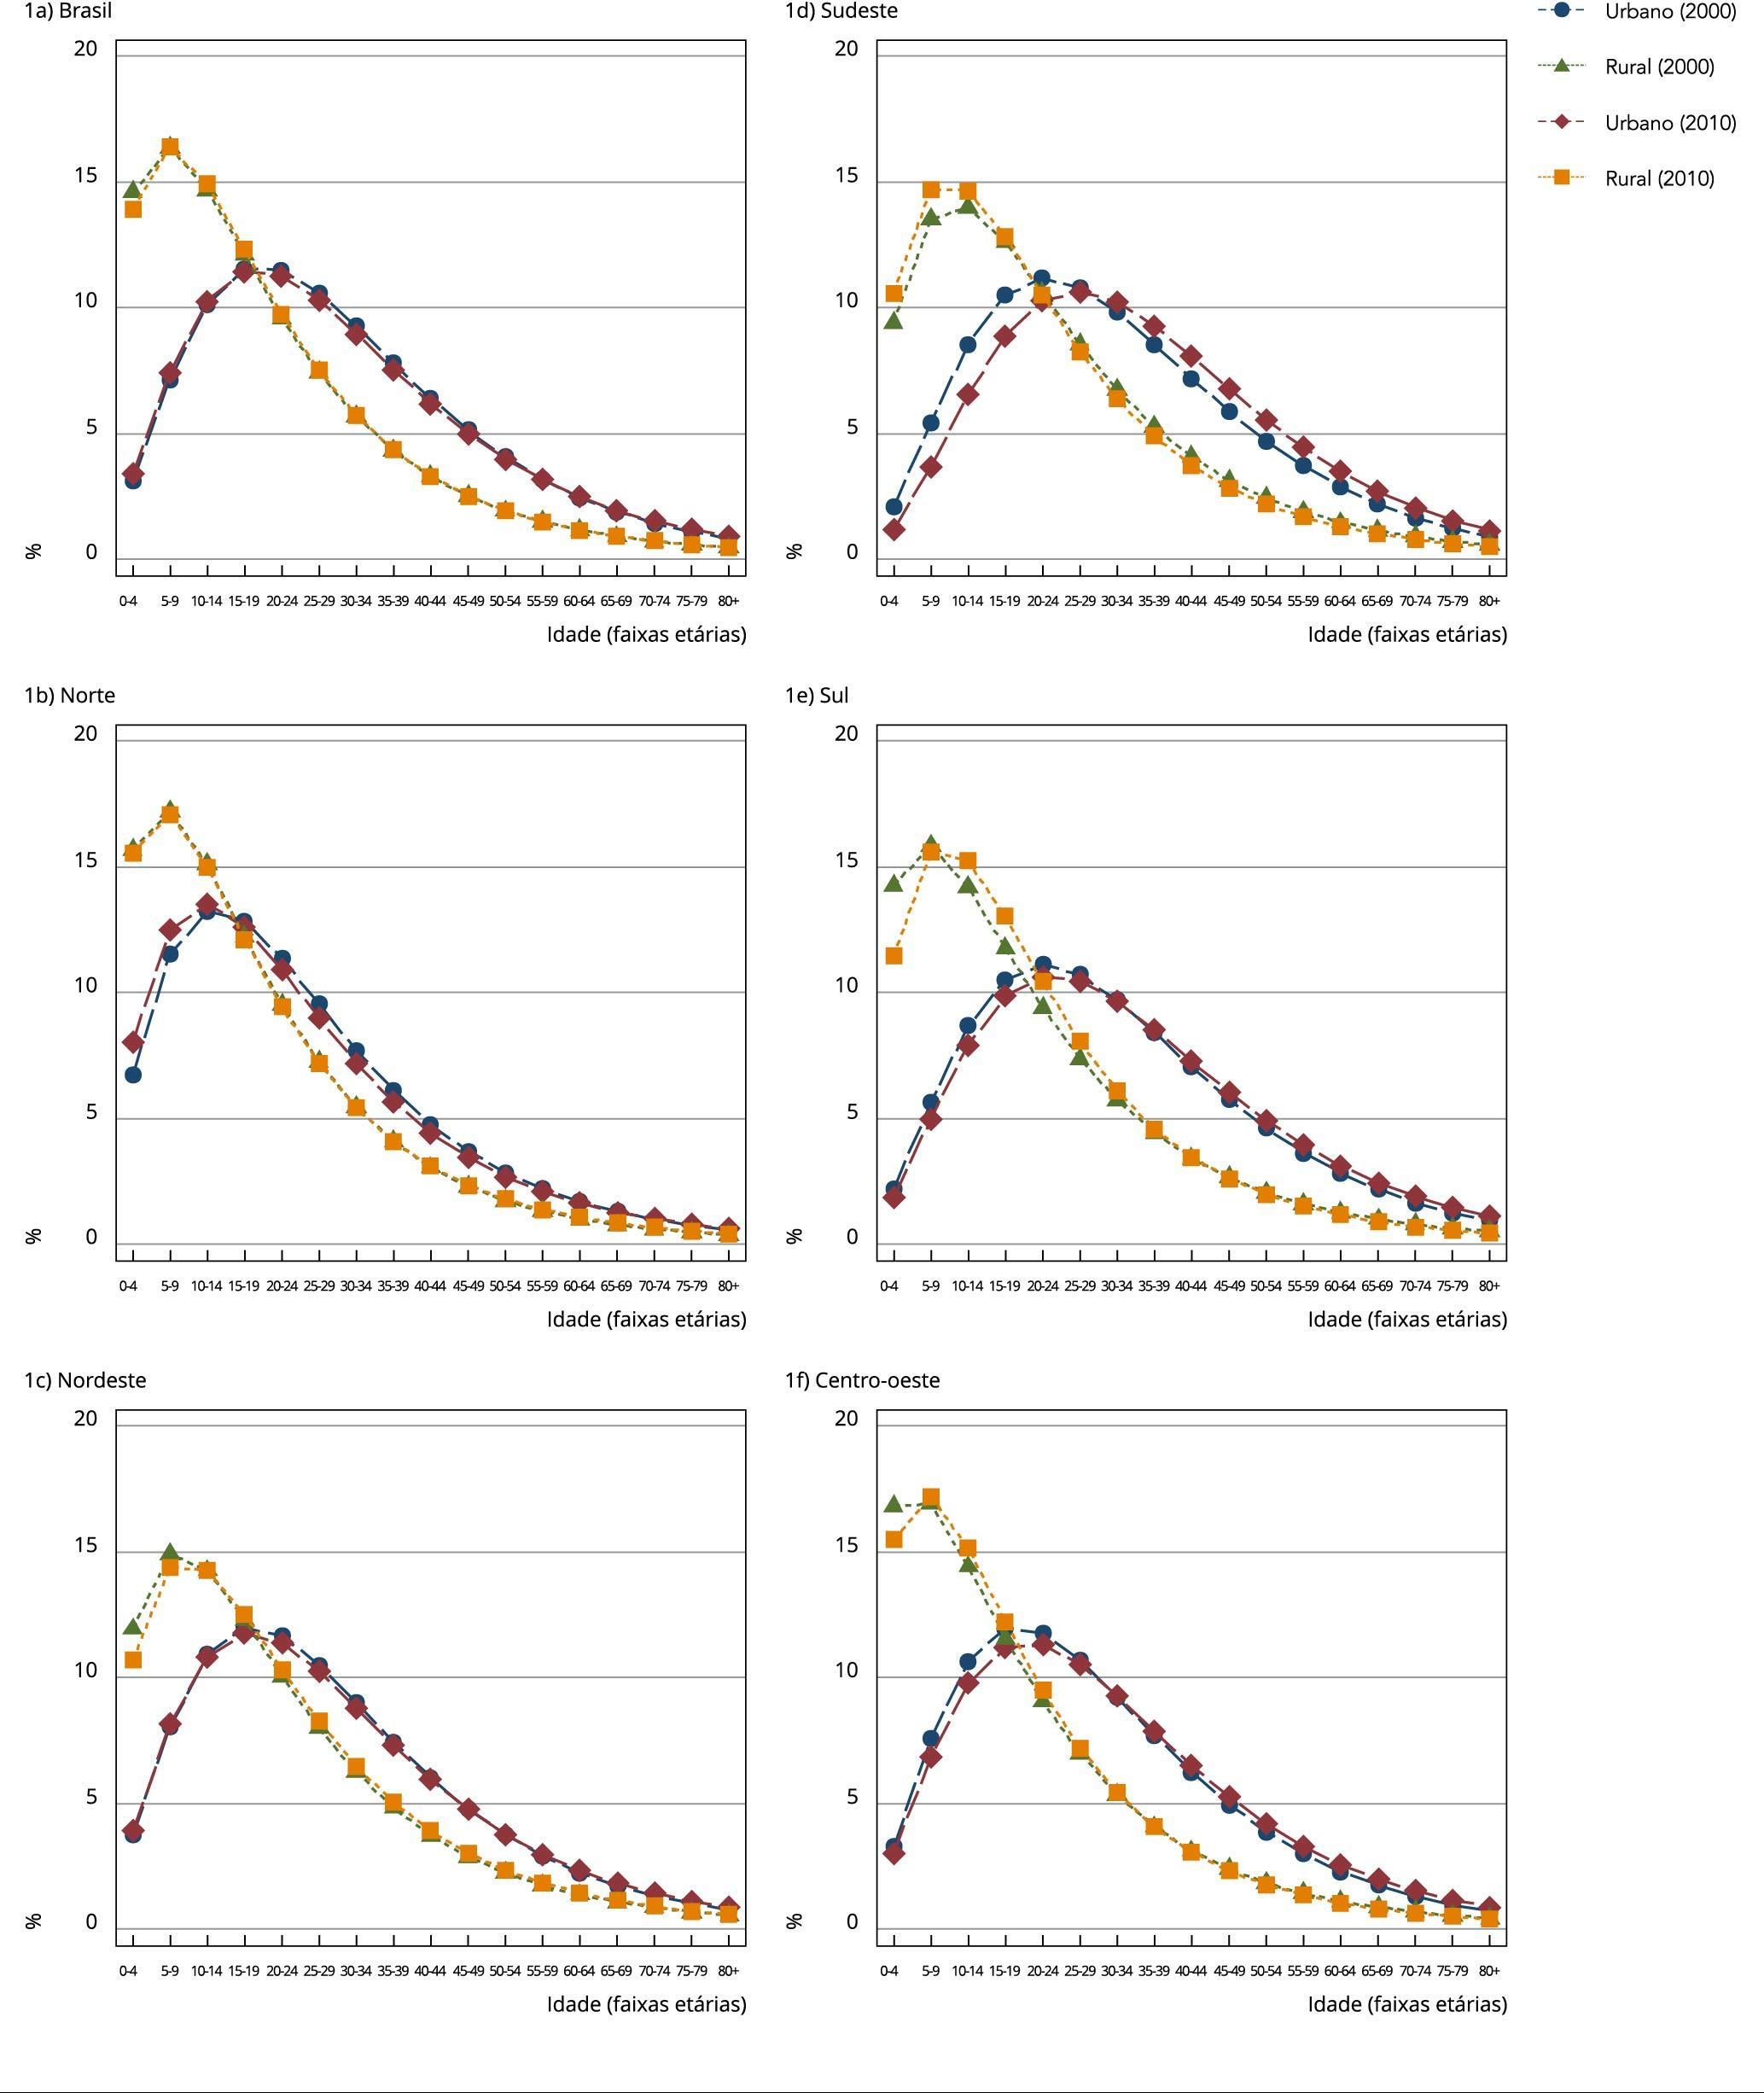
\includegraphics[width=\textwidth]{1678-4464-csp-33-s1-e00085516-gf1.jpg}
\caption{}\label{fig:f1}
\end{figure}

O grau de escolarização dos indígenas entre 2000 e 2010, apresentado na Figura~\ref{fig:f2}, aumentou no período, sendo observada maior participação relativa da categoria
de Ensino Fundamental completo ou mais e, consequentemente, menor expressão do
grupo com até Ensino Fundamental incompleto. As variações entre macrorregiões e
áreas urbanas ou rurais indicadas nas tabelas se mantiveram nos resultados dessa
figura. Com relação à renda (Figura~\ref{fig:f3}
), observou-se estabilidade dos indivíduos sem rendimento, aumento proporcional
da categoria com até 1 salário mínimo, manutenção da frequência do grupo com 1-2
salários mínimos e redução percentual da faixa com mais de 2 salários mínimos.
Salientam-se, novamente, as inexpressivas diferenças entre áreas urbanas e
rurais em todas as macrorregiões do país.

\begin{figure}
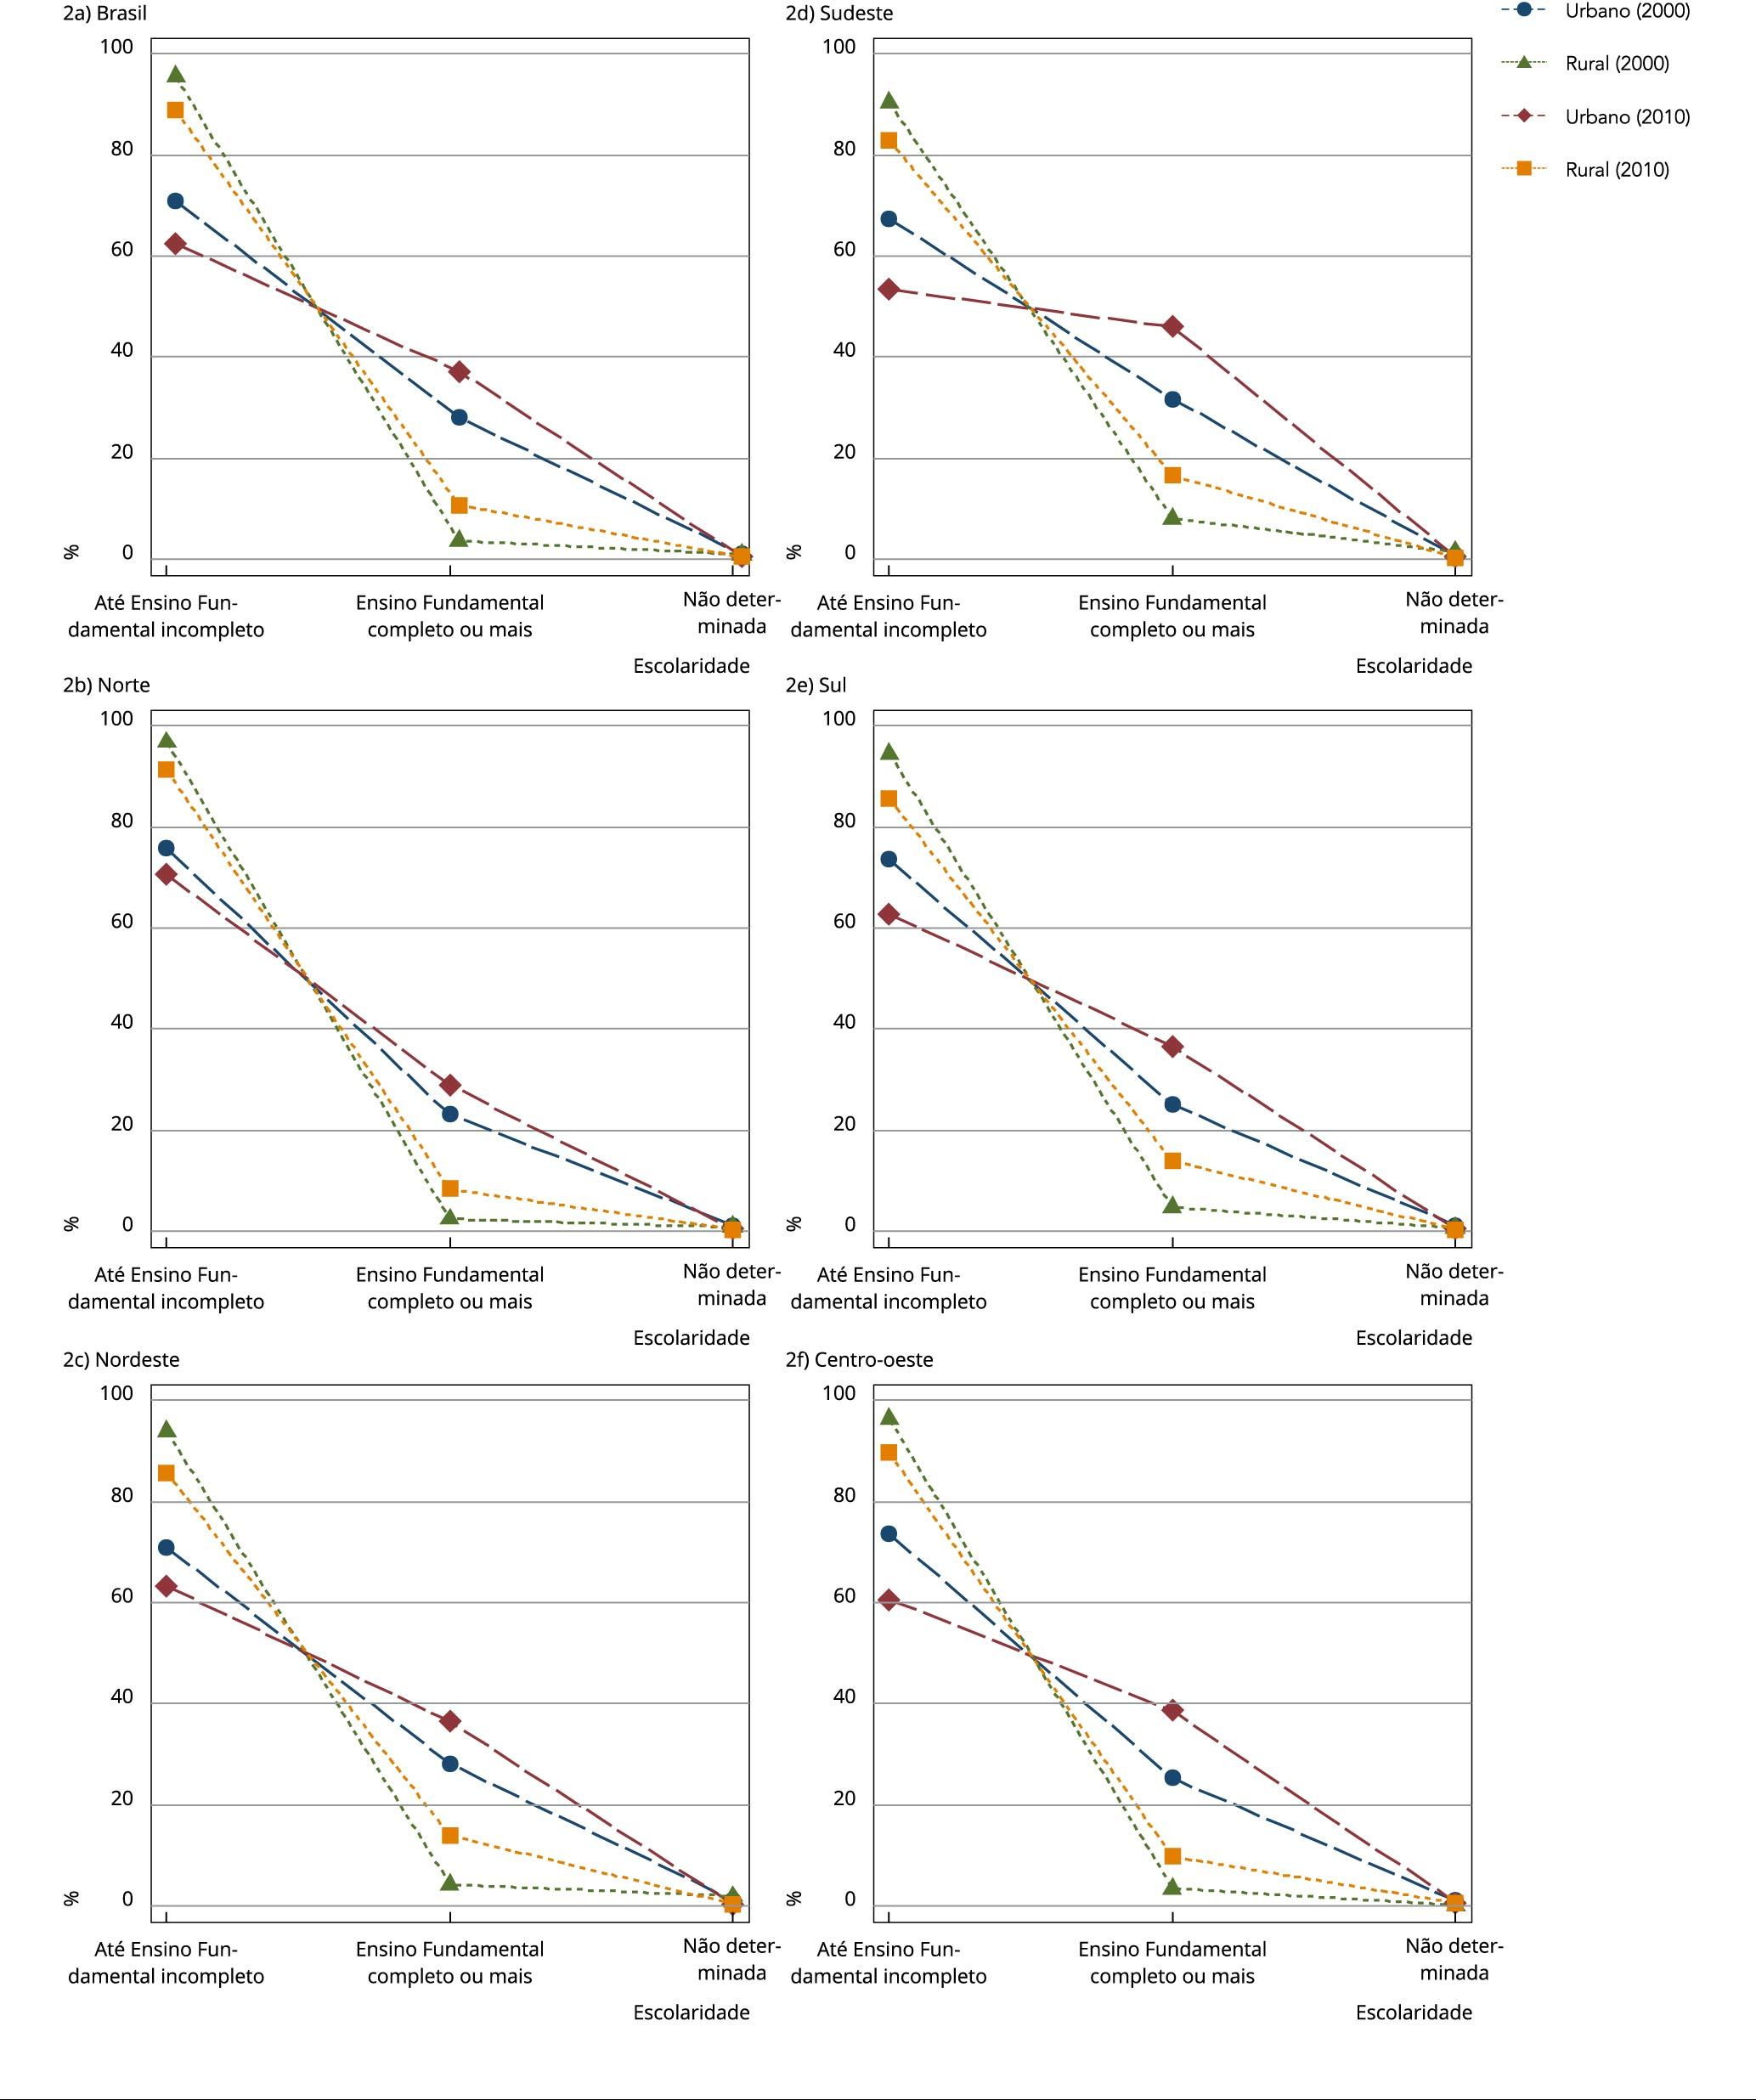
\includegraphics[width=\textwidth]{1678-4464-csp-33-s1-e00085516-gf2.jpg}
\caption{}\label{fig:f2}
\end{figure}

\begin{figure}
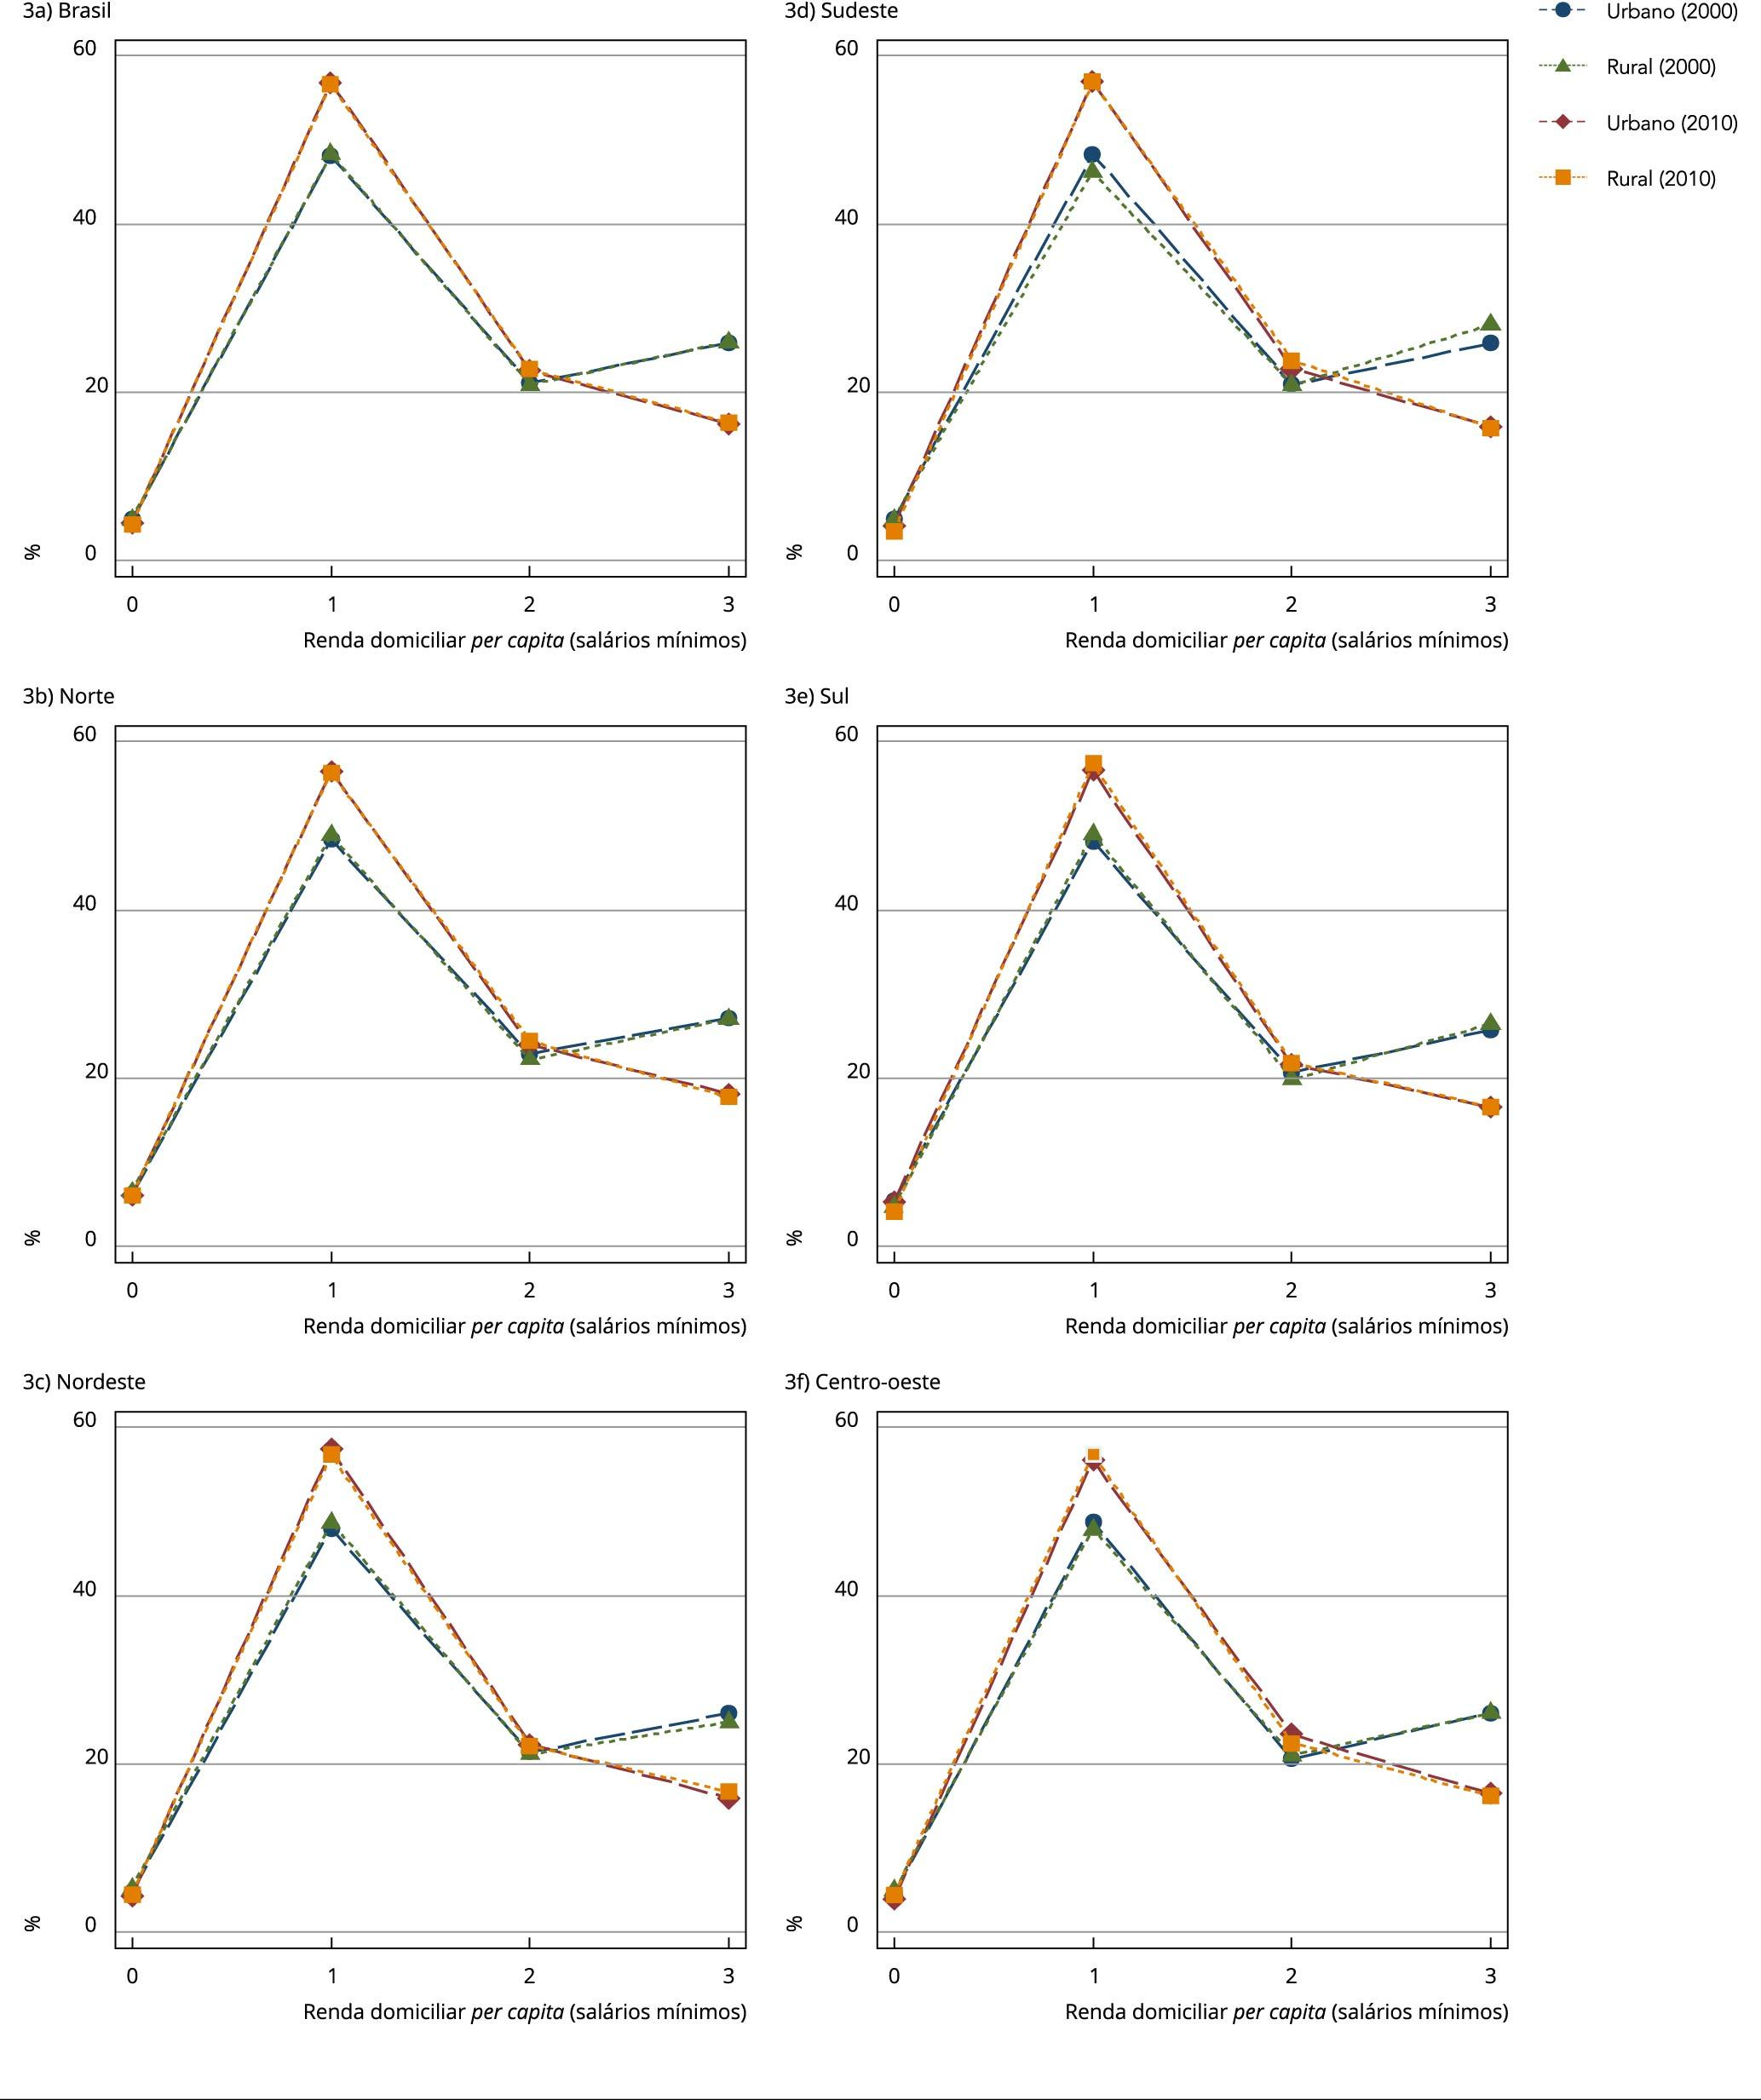
\includegraphics[width=\textwidth]{1678-4464-csp-33-s1-e00085516-gf3.jpg}
\caption{}\label{fig:f3}
\end{figure}

Por fim, a Figura~\ref{fig:f4}
demonstrou que a contagem do total de moradores nos domicílios reduziu, em
média, ao longo do período. Além disso, essa figura igualmente sugere que as
distribuições do total de moradores nos domicílios não diferiram, se comparadas
as áreas urbanas com as rurais internamente a cada ano censitário.

\begin{figure}
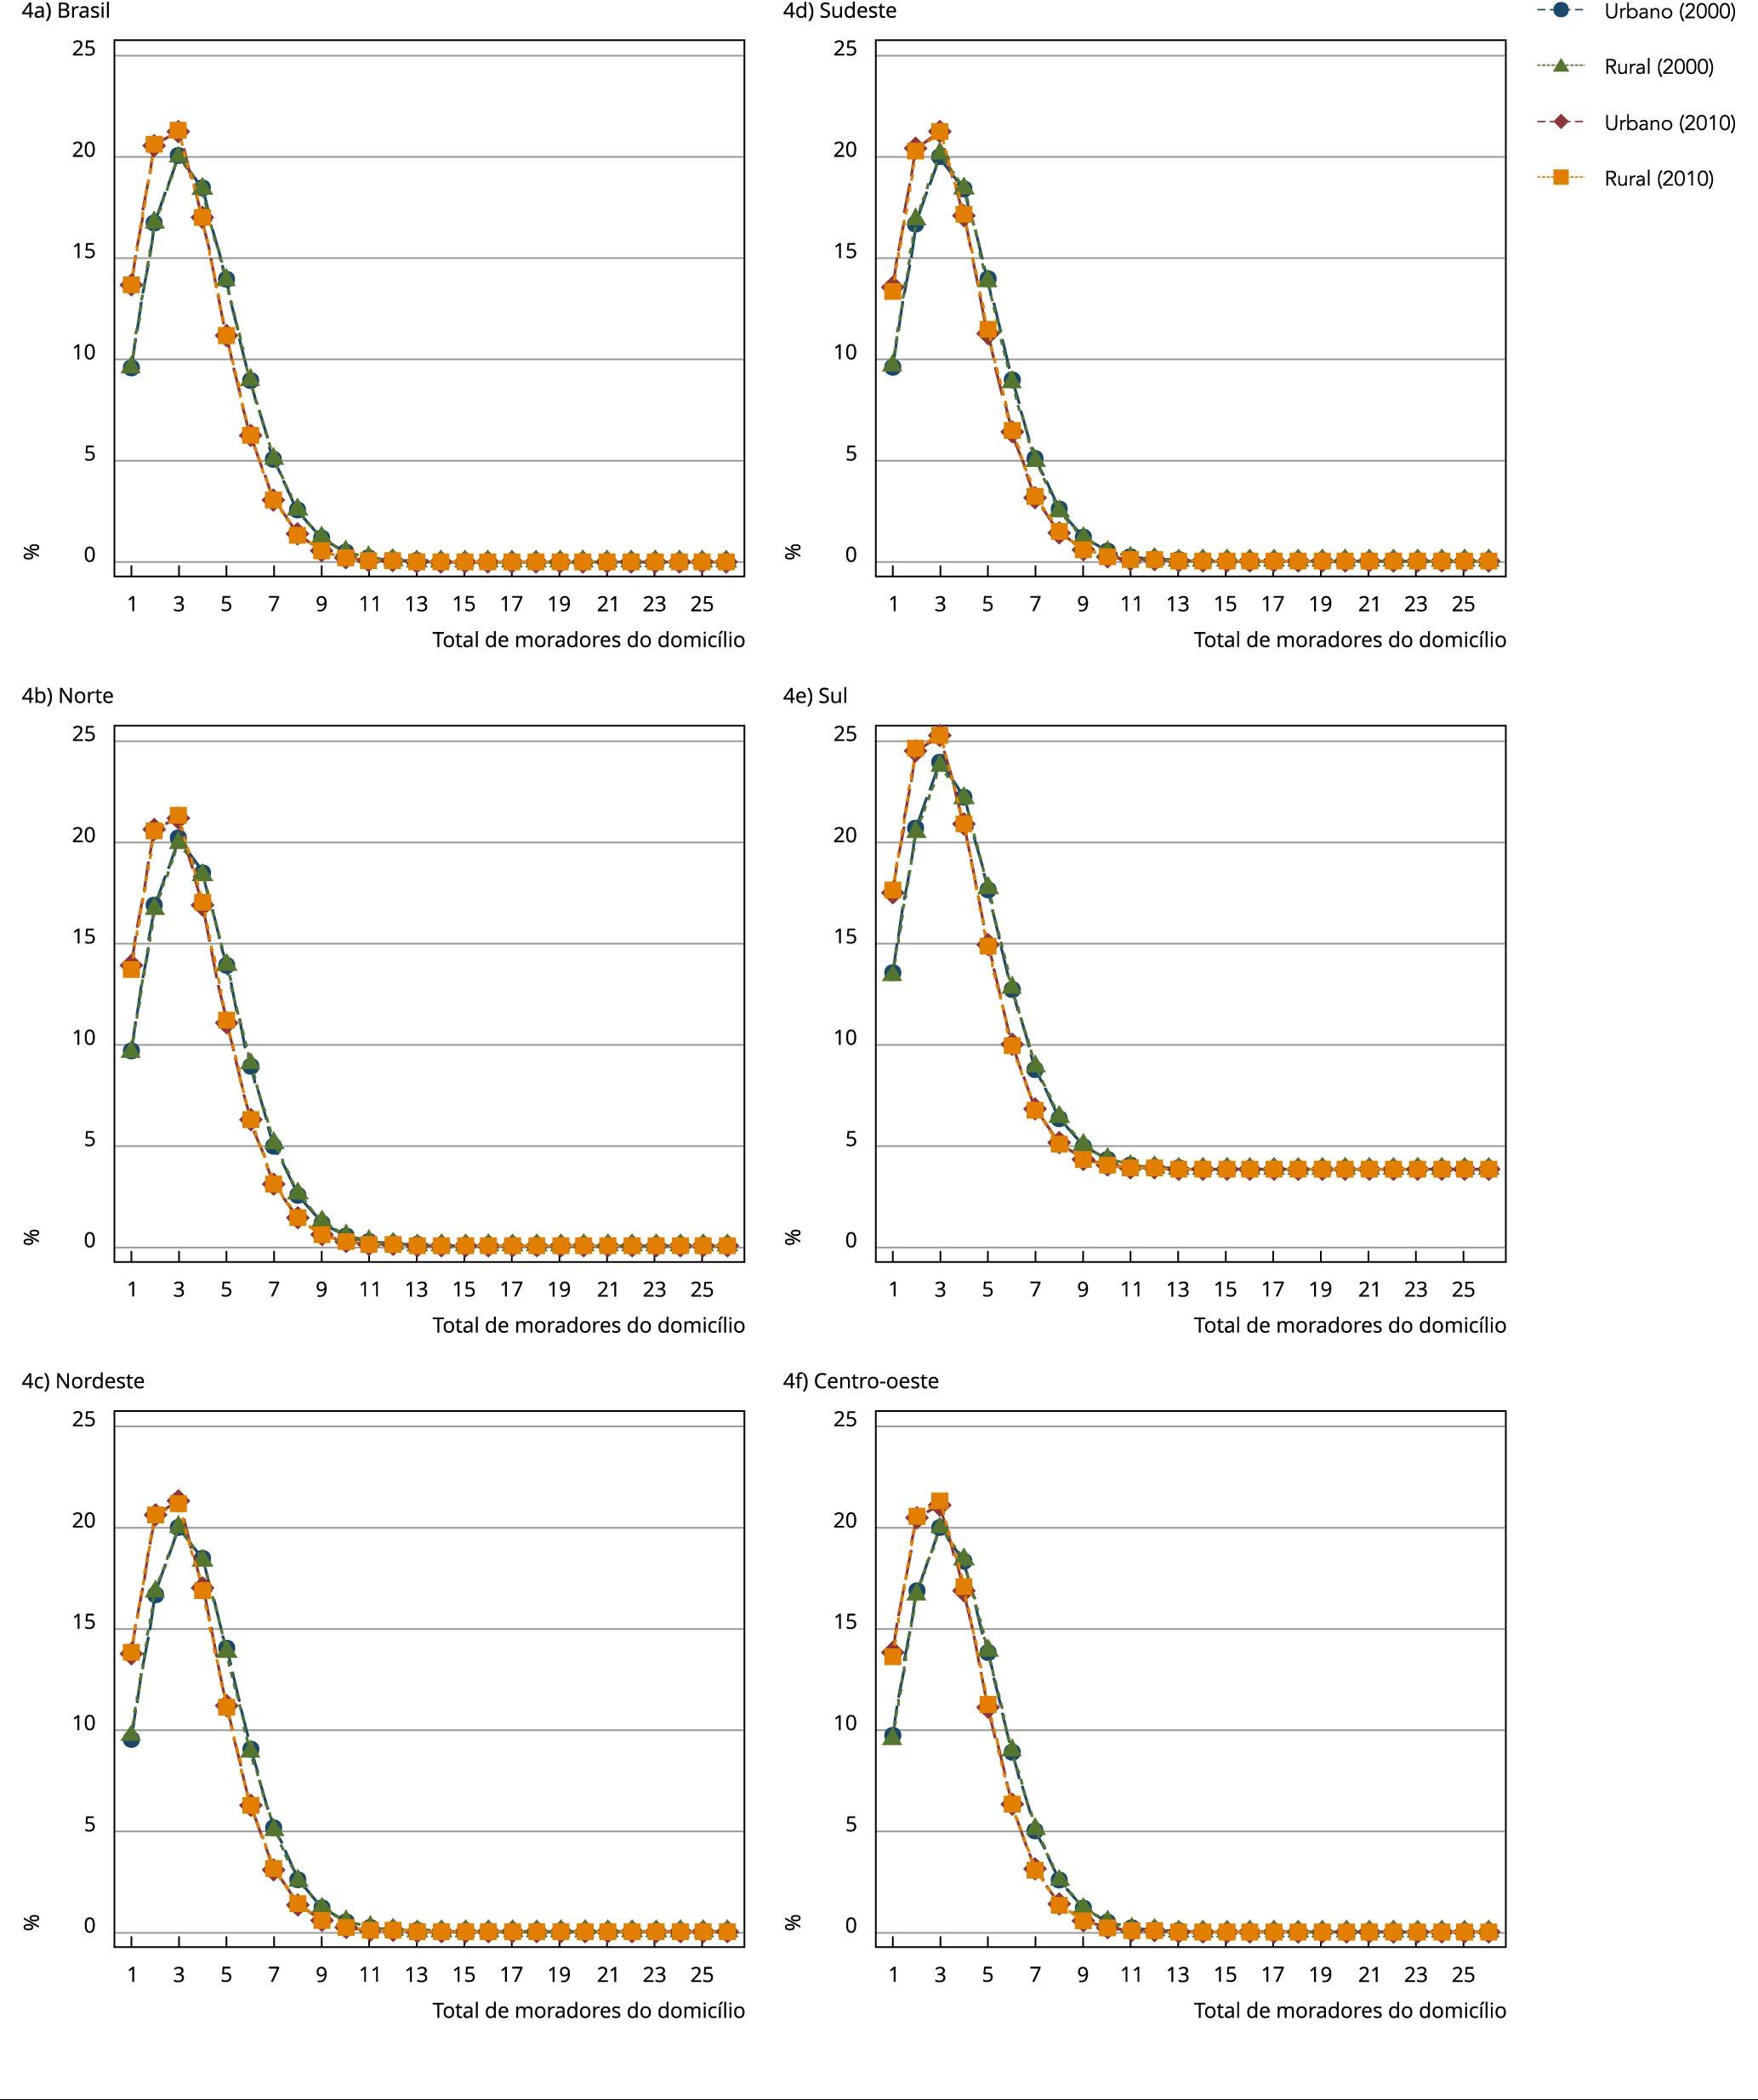
\includegraphics[width=\textwidth]{1678-4464-csp-33-s1-e00085516-gf4.jpg}
\caption{}\label{fig:f4}
\end{figure}

\section{Discussão}

A partir da divulgação dos dados do Censo 2010, vêm sendo publicadas análises
comparativas envolvendo recenseamentos anteriores, com destaque para o 2000\textsuperscript{[}\textsuperscript{7}\textsuperscript{]}\textsuperscript{,}\textsuperscript{[}\textsuperscript{8}\textsuperscript{]}\textsuperscript{,}\textsuperscript{[}\textsuperscript{11}\textsuperscript{]}. O expressivo crescimento da população indígena entre 1991 e 2000, conforme
aludido na \textit{Introdução}, tem sido atribuído a um cenário mais amplo de (re)emergência de etnicidades
indígenas em um contexto de valorização e reconhecimento da sociodiversidade
presente no país no período seguinte à promulgação da \textit{Constituição
Federal}
de 1988. Por outro lado, ao se comparar 2000 com 2010, uma das principais
questões abordadas em estudos sociodemográficos tem sido buscar explicações para
a inesperada variação no tamanho da população indígena entre os dois censos, em
particular a redução na área urbana\textsuperscript{[}\textsuperscript{11}\textsuperscript{]}. Uma linha explicativa é que, com a inclusão de perguntas sobre etnia e língua
falada no domicílio em 2010, é possível que menos respondentes, sobretudo nas
regiões urbanas do Sul e do Sudeste, tenham optado pela categoria indígena no
quesito cor/raça. Não há estudos antropológicos detalhados sobre o tema, mas é
factível supor que, no contexto do levantamento censitário, a noção de
pertencimento indígena tenha se atrelado a ter etnia específica e/ou falar
língua indígena. De qualquer forma, para além da compreensão da variação desses
contingentes populacionais, outra linha de pesquisa menos enfatizada é a
investigação comparativa das características demográficas e socioeconômicas dos
indígenas em 2000 e 2010. Nesse caso, o estudo mais detalhado foi realizado pelo
\textsc{ibge} e enfocou, entre outros aspectos, distribuição regional e urbano/rural,
alfabetização, rendimentos e saneamento\textsuperscript{[}\textsuperscript{7}\textsuperscript{]}\textsuperscript{,}\textsuperscript{[}\textsuperscript{11}\textsuperscript{]}.

O presente trabalho está inserido no conjunto de esforços voltados para abordar
comparativamente os resultados acerca de indígenas nos censos de 2000 e 2010. Em
relação às investigações já realizadas, além de detalhar similaridades e
diferenças entre as características demográficas e socioeconômicas dos indígenas
com base em frequências absolutas e relativas simples, este estudo inova pelo
uso de modelos de regressão com vistas ao ajuste para covariáveis. A importância
dessa abordagem pode ser evidenciada por meio de um exemplo: análises
anteriores, inclusive estudos conduzidos pelo \textsc{ibge}, já haviam apontado para o
fato de que, no Brasil como um todo e também em suas macrorregiões, houve um
aumento nas taxas de alfabetização de indígenas com 15 anos de idade e mais
entre 2000 e 2010\textsuperscript{[}\textsuperscript{7}\textsuperscript{]}. Não obstante, a interpretação dessa informação precisa levar em consideração
que houve mudanças na estrutura etária dos indígenas no período. Nesse sentido,
as modelagens estatísticas são úteis no sentido de auxiliar na interpretação dos
dados, levando-se em consideração outras características que afetam a
comparação, dentre as quais a composição etária do segmento analisado.

As análises aqui detalhadas reforçam um conjunto de tendências para os indígenas
entre 2000 e 2010. Em consonância com estudos prévios\textsuperscript{[}\textsuperscript{7}\textsuperscript{]}\textsuperscript{,}\textsuperscript{[}\textsuperscript{8}\textsuperscript{]}, além de as mudanças no tamanho da população indígena indicarem variações
importantes entre os dois censos, foram observadas alterações significativas nas
distribuições regionais ao se abordar as situações urbana e rural. No caso das
áreas rurais, especificamente, houve aumento da população indígena entre 2000 e
2010, de 347.145 para 494.306 indivíduos, mas o perfil geral de distribuição
proporcional entre as macrorregiões praticamente não se alterou. Em ambos os
censos, o Norte rural concentrava cerca de 50\% da população, com o Nordeste e o
Centro-oeste apresentando proporções de 20\% cada, perfazendo cerca de 90\% do
total de indígenas vivendo em situação rural no país. Por sua vez, o cenário de
alterações nas áreas urbanas se mostrou mais heterogêneo, uma vez que a redução
de sua população indígena (de 379.560 em 2000 para 318.769 em 2010) foi
acompanhada por expressivas transformações nas distribuições regionais. Enquanto
algumas macrorregiões experimentaram aumentos tanto absolutos como relativos
(e.g., Norte e Nordeste), outras, como o Sudeste e o Sul, passaram a apresentar
menores quantitativos, absolutos e relativos, em 2010. Ao se considerar as
diferenças nas proporções da população indígena no tocante à macrorregião e
situação urbano/rural, as transformações mais expressivas entre os dois censos,
da ordem de 5 p.p. ou mais, ocorreram em apenas três estratos: Sudeste urbano
(36,7\% em 2000 \textit{vs.}
25,5\% em 2010), Nordeste urbano (27,6\% \textit{vs.}
33,8\%) e Norte urbano (12,1\% \textit{vs.}
19\%).

Ainda que não descartando as influências de outros fatores (como a maior ou
menor propensão à declaração em uma dada categoria de cor ou raça, ou a
crescente urbanização do país e as possíveis mudanças na demarcação de áreas
urbanas e rurais pelos municípios brasileiros entre 2000 e 2010), as variações
no volume da população indígena em área rural, com uma taxa média geométrica de
crescimento anual de 3,7 entre 2000 e 2010\textsuperscript{[}\textsuperscript{11}\textsuperscript{]}, são potencialmente explicáveis pela dinâmica demográfica propriamente, em
particular a relação entre níveis de natalidade e mortalidade, assim como
migração, esta última talvez em menor escala\textsuperscript{[}\textsuperscript{17}\textsuperscript{]}. Por sua vez, sobretudo no cenário de redução da população indígena em área
urbanas, é menos plausível explicar as transformações sem considerar a
possibilidade de influências mais incisivas relacionadas a procedimentos de
captação de dados e mudanças nas perspectivas de reconhecimento étnico-racial.
Por exemplo, conforme já mencionado, se a declaração sobre pertencimento
indígena no Censo 2000 derivou unicamente da resposta à pergunta sobre cor ou
raça, em 2010 foram incluídas questões sobre filiação étnica específica (povo ou
etnia indígena) e línguas faladas nos domicílios\textsuperscript{[}\textsuperscript{7}\textsuperscript{]}. É possível que entrevistados residentes em área urbana que optaram pela
categoria indígena em 2000 possam ter deixado de fazê-lo em 2010, especialmente
em função de serem confrontados com perguntas sobre etnia e língua falada no
domicílio, conforme já aventado. Esse efeito pode ter sido potencializado em
algumas regiões do país, com destaque para o Sudeste urbano.

Ressalte-se que a questão das inter-relações entre fatores demográficos e
dimensões sociopolíticas influenciando o perfil de cor ou raça é algo mais geral
no país, e mesmo em outros países, não se restringindo às minorias indígenas\textsuperscript{[}\textsuperscript{18}\textsuperscript{]}\textsuperscript{,}\textsuperscript{[}\textsuperscript{19}\textsuperscript{]}. Nesse sentido, Miranda\textsuperscript{[}\textsuperscript{20}\textsuperscript{]}
argumenta que variações recentes nas proporções de pessoas de cor ou raça preta
e parda no Brasil, com tendência de aumento entre 2000 e 2010, possivelmente se
vinculam à implantação de políticas públicas de ação afirmativa de recorte
racial nos últimos anos (ver também Telles\textsuperscript{[}\textsuperscript{19}\textsuperscript{]}
e Francis \& Tannuri-Pianto\textsuperscript{[}\textsuperscript{21}\textsuperscript{]}\textsuperscript{,}\textsuperscript{[}\textsuperscript{22}\textsuperscript{]}
). No caso da população indígena, com base nos dados censitários, é importante
considerar que a classificação no recorte da cor ou raça se entrecruza com
dimensões ligadas à etnia e à língua, além de toda uma pletora de aspectos
socioeconômicos, resultando em complexos processos classificatórios com
características ainda muito pouco conhecidas\textsuperscript{[}\textsuperscript{3}\textsuperscript{]}\textsuperscript{,}\textsuperscript{[}\textsuperscript{8}\textsuperscript{]}\textsuperscript{,}\textsuperscript{[}\textsuperscript{10}\textsuperscript{]}\textsuperscript{,}\textsuperscript{[}\textsuperscript{15}\textsuperscript{]}\textsuperscript{,}\textsuperscript{[}\textsuperscript{23}\textsuperscript{]}.

Considerando o conjunto de resultados detalhados no presente estudo, talvez o
que mais chame atenção sejam as tendências convergentes observadas nas
características sociodemográficas da população indígena, a despeito das já
referidas variações (positivas e negativas) nos volumes de população segundo
recortes rural/urbano e macrorregiões. Por exemplo, Sudeste e Nordeste urbanos
experimentaram mudanças distintas, com redução (36,7\% para 25,5\%) e aumento
(27,6\% e 33,8\%) nas proporções em relação ao total no país, respectivamente.
Ao mesmo tempo, o padrão geral de alteração nos perfis de escolaridade, renda
domiciliar e número de moradores por domicílio entre os estratos foi semelhante
para as duas macrorregiões. Nesse sentido, ainda que haja particularidades
regionais, os achados das análises de regressão não evidenciaram recortes
(macrorregião segundo urbano/rural) com padrões de mudanças marcadamente
dissonantes em relação aos observados em geral. Isso incluiu tendência de
envelhecimento (mais leve nas áreas rurais e um pouco mais pronunciada no
Sudeste, Sul e Centro-oeste urbanos); aumento da escolaridade (em particular na
faixa do Ensino Fundamental completo ou mais); diminuição de domicílios sem
renda, assim como daqueles com > 2 salários mínimos; e redução no número de
moradores nos domicílios. Vale indicar que tais mudanças na direção do
envelhecimento populacional, aumento de escolaridade e renda, e redução no
número de moradores nos domicílios, vêm também, grosso modo, sendo observadas na
população brasileira em geral, ainda que com intensidades e temporalidades
distintas\textsuperscript{[}\textsuperscript{24}\textsuperscript{]}.

Diante do exposto, depreende-se que, surpreendentemente, os padrões
diferenciados de ganho ou a perda de população indígena não fizeram com que
macrorregiões específicas, segundo recorte urbano ou rural, tendessem a se
particularizar ainda mais quanto aos perfis de transformações sociodemográficas.
Sejam quais forem as explicações para as variações nos volumes de indígenas
entre os dois censos, incluindo a já referida possibilidade de menor adesão à
categoria indígena nos centros urbanos do Sul/Sudeste devido aos aspectos de
filiação étnica específica e língua falada, não resultou em variações
marcadamente diferenciadas nos perfis sociodemográficos ao se comparar as
diversas regiões, tanto aquelas nas quais houve redução como aumento de
população. Se a explicação para a redução da população indígena urbana entre
2000 e 2010 já se constituía um importante desafio analítico, sugeriríamos que a
questão associada da convergência nos perfis socioeconômicos tanto nos contextos
de perda como de ganho de população indígena também seja priorizada nas
pesquisas sobre demografia indígena com base nos dados censitários.

Os resultados de renda domiciliar \textit{per capita}
entre 2000 e 2010 também se revelaram de difícil compreensão, na medida em que
todas as categorias apresentaram proporções semelhantes nas macrorregiões
analisadas, tanto em áreas urbanas quanto rurais. Ademais, os ganhos na faixa de
até 1 salário mínimo foram contrabalançados pela redução proporcional do grupo
com mais do que 2 salários mínimos. Não se pode descartar a possibilidade de que
a aferição dos rendimentos domiciliares implique complexidade adicional no caso
dos indígenas, especialmente aqueles localizados em áreas rurais e que não têm o
Português como língua materna. Análise prévia de dados censitários\textsuperscript{[}\textsuperscript{15}\textsuperscript{]}
indicou, por exemplo, que as mães indígenas da Região Norte apresentaram
elevados percentuais de respostas dadas ao recenseador por outra pessoa, que não
elas próprias, acerca da quantidade de filhos que tiveram ao longo de suas vidas
reprodutivas. Em conjunto, esses resultados sinalizam para uma complexidade de
fatores de ordem sociocultural que podem interferir na produção de dados
censitários em geral (e não somente daqueles vinculados à renda), tornando
intricada a intepretação dos padrões e perfis deles derivados.

Por sua vez, a redução do número de moradores nos domicílios indígenas, apesar
de consistente e homogênea ao longo das macrorregiões e situações urbanas ou
rurais, se deparou com uma relativa inércia na estrutura etária de 2000 para
2010. Isso é particularmente inesperado, visto que a diminuição no total de
moradores nos domicílios deveria estar, a rigor, vinculada ao envelhecimento da
estrutura etária da população. Dado que apenas o Sudeste urbano se destacou como
estrato com perceptível, mas sutil, alteração na distribuição etária,
esperava-se que a contagem média de moradores reduzisse em maior intensidade ao
ser comparado com as demais macrorregiões. Marinho\textsuperscript{[}\textsuperscript{25}\textsuperscript{]}
apontou expressiva redução da quantidade de domicílios indígenas nas áreas
urbanas (de cerca de 134.000 em 2000 para 112.000 em 2010), bem como aumento nas
rurais (partindo de 66.000 em 2000 e atingindo 96.000 em 2010). Isso é, a
pulverização dos indígenas em um maior número de domicílios na área rural
explicaria apenas parcialmente a redução de moradores nas residências indígenas,
visto que o mesmo não foi registrado para as áreas urbanas. Uma hipótese a ser
avaliada é se, por exemplo, as reduções observadas entre 2000 e 2010, em
particular nas áreas urbanas do Sudeste e Sul, foram mais pronunciadas no caso
de indivíduos indígenas que residiam em domicílios nos quais os demais
moradores, incluindo o responsável, não eram indígenas. Uma alteração como essa
se alinharia com os achados do presente estudo, no sentido de padrões de
alteração diferenciados nos volumes de população, seja aumento ou diminuição,
acompanhados de mudanças em perfis socioeconômicos que não se destacaram como
marcadamente distintos segundo macrorregiões e contextos urbano/rural.

Em conclusão, o conjunto desses resultados é indicativo de tendências relevantes
para o segmento indígena residente no Brasil em um intervalo de dez anos. Ao
mesmo tempo, tais resultados se impõem com particular complexidade e desafio
face às iniciativas de compreensão. Esses aspectos podem desembocar em questões,
por exemplo, de natureza metodológica, se considerarmos os instrumentos e o
trabalho de campo envolvidos nas coletas censitárias: (1) Considerando a
magnitude de redução populacional no Sudeste e, em paralelo, seu relativo
envelhecimento, estaríamos tratando da mesma população indígena tanto em 2000
quanto em 2010? (2) Embora o país seja marcado por desigualdades macrorregionais
e urbano/rurais, como explicar mudanças em geral semelhantes nas distribuições
de renda e de número de moradores nos domicílios ao longo dos 10 anos?
Indubitavelmente, esses questionamentos acenam para a necessidade de análises
mais aprofundadas das tendências populacionais aqui observadas que, inclusive,
sejam amparadas em dados que ainda estão por ser produzidos nas próximas edições
do censo demográfico brasileiro. Afinal, qualquer análise de tendência
demográfica requer a disponibilidade de dados coletados em múltiplos pontos no
tempo, e não somente dois. Reforça-se assim que, sendo os indígenas um dos
segmentos étnico-raciais de maior vulnerabilidade socioambiental no país, há
necessidade de que as análises aqui apresentadas tenham continuidade e
aprofundamento. Isso será imprescindível para que as tendências sejam
acompanhadas e para que sejam avaliadas e implantadas políticas públicas
direcionadas a esse segmento populacional.

Agradecimentos
João Luiz Bastos e Ricardo Ventura Santos agradecem ao Conselho Nacional de
Desenvolvimento Científico e Tecnológico (\textsc{cnp}q) por concessão de bolsa de
produtividade em pesquisa (processos nº 303857/2015-3 e nº 304358/2014-2,
respectivamente). Agradecemos também o financiamento à pesquisa da Fundação de
Amparo à Pesquisa do Estado do Rio de Janeiro (Faperj; projeto nº
E-26/102.352/2013).

\section*{Referências}
\begin{itemize}

\item[1] United Nations. State of the world's indigenous peoples. New York:
United Nations; 2009.

\item[2] Loveman M. National colors: racial classification and the state in
Latin America. Oxford: Oxford University Press; 2014.

\item[3] Del Popolo F, Cunha EP, Ribotta B, Azevedo M. Pueblos indígenas y
afrodescendientes en América Latina: dinámicas poblacionales diversas y desafios
comunes. Rio de Janeiro: \textsc{alap} Editor; 2011.

\item[4] Del Popolo F. Los pueblos indígenas y afrodescendientes en las
fuentes de datos: experiencias en América Latina. Santiago: Comisión Económica
para América Latina y el Caribe; 2008.

\item[5] Ministério da Saúde. Política Nacional de Atenção à Saúde dos Povos
Indígenas. Brasília: Ministério da Saúde; 2000.

\item[6] Cardoso AM, Santos RV, Coimbra Jr. \textsc{cea}, Garnelo L, Chaves \textsc{mbg}.
Políticas públicas de saúde para os povos indígenas. In: Giovanella L, Escorel
S, Lobato \textsc{lvc}, Noronha JC, Carvalho AI, organizadores. Políticas e sistemas de
saúde no Brasil. Rio de Janeiro: Editora Fiocruz; 2012. p. 911-32.

\item[7] Instituto Brasileiro de Geografia e Estatística. Censo demográfico
2010: características gerais dos indígenas, resultados do universo. Rio de
Janeiro: Instituto Brasileiro de Geografia e Estatística; 2012.

\item[8] Azevedo MM. O censo 2010 e os povos indígenas. In: Ricardo CA,
Ricardo F, editores. Povos indígenas do Brasil 2006/2010. São Paulo: Instituto
Socioambiental; 2011. p. 25-45.

\item[9] Pagliaro H, Azevedo MM, Santos RV. Demografia dos povos indígenas no
Brasil. Rio de Janeiro: Editora Fiocruz/Associação Brasileira de Estudos
Populacionais; 2005.

\item[10] Santos RV, Teixeira P. O "indígena" que emerge do Censo
Demográfico de 2010. Cad Saúde Pública 2011; 27:1048-9.

\item[11] Instituto Brasileiro de Geografia e Estatística. Os indígenas no
Censo Demográfico 2010: primeiras considerações com base no quesito cor ou raça.
Rio de Janeiro: Instituto Brasileiro de Geografia e Estatística; 2012.

\item[12] Gonçalves \textsc{jmm}. \textsc{ibge}: um retrato histórico. Rio de Janeiro:
Instituto Brasileiro de Geografia e Estatística; 1995.

\item[13] Instituto Brasileiro de Geografia e Estatística. Estatísticas do
século XX. Rio de Janeiro: Instituto Brasileiro de Geografia e Estatística;
2006.

\item[14] Instituto Brasileiro de Geografia e Estatística. Metodologia do
censo demográfico 2010. Rio de Janeiro: Instituto Brasileiro de Geografia e
Estatística; 2013.

\item[15] Ventura Santos R, Luiz Bastos J, Gonçalves Cruz O, de Barros Longo
LA, Flowers NM, de Oliveira Martins Pereira N. Parity of indigenous and
non-indigenous women in Brazil: does the reported number of children born depend
upon who answers national census questions? PLoS One 2015; 10:e0123826.

\item[16] Long JS, Freese J. Regression models for categorical dependent
variables using Stata. College Station: Stata Press; 2014.

\item[17] Instituto Brasileiro de Geografia e Estatística. Censo demográfico
2010: nupcialidade, fecundidade e migração. Resultados da amostra. Rio de
Janeiro: Instituto Brasileiro de Geografia e Estatística; 2010.

\item[18] Roth WD. The multiple dimensions of race. Ethn Racial Stud 2016;
39:1310-38.

\item[19] Telles E. Demography of race in Brazil. In: Saénz R, Embrick DG,
Rodríguez N, editors. The international handbook of the demography of race and
ethnicity. New York: Springer; 2015. p. 151-67.

\item[20] Miranda V. A resurgence of black identity in Brazil? Evidence from
an analysis of recent censuses. Demogr Res 2015; 32:1603-30.

\item[21] Francis AM, Tannuri-Pianto M. Using Brazil's racial continuum to
examine the short-term effects of affirmative action in higher education. J Hum
Resour 2012; 47:754-84.

\item[22] Francis AM, Tannuri-Pianto M. Endogenous race in Brazil:
affirmative action and the construction of racial identity among young adults.
Econ Dev Cult Change 2013; 61:731-53.

\item[23] Oliveira JP. Mensurando alteridades, estabelecendo direitos:
práticas e saberes governamentais na criação de fronteiras étnicas. Dados 2012;
55:1055-88.

\item[24] Instituto Brasileiro de Geografia e Estatística. Tendências
demográficas: uma análise dos indígenas com base nos resultados da amostra dos
censos demográficos 1991 e 2000. Rio de Janeiro: Instituto Brasileiro de
Geografia e Estatística; 2005.

\item[25] Marinho GL. Domicílios indígenas nos censos demográficos:
classificação, composição e interfaces com a saúde [Tese de Doutorado]. Rio de
Janeiro: Fundação Oswaldo Cruz; 2015.

\end{itemize}

\end{document}
